\chapter{Stand der Technik}
\label{cha:Stand der Technik}



Dieses Kapitel gibt einen Überblick über den aktuellen Stand der Wissenschaft und Technik im Bezug auf :
\begin{itemize}
\item Untersuchungen zur Eisbildung auf Luftkühlern
\item Abtaumethoden und -messungen von Luftkühlern.
\end{itemize}

%\newpage
\section{Abtaumethoden}
\label{sec: Abtaumethoden}

Um einen vereisten Luftkühler abzutauen, gibt es mehrere Methoden. Die Methoden unterscheiden sich in Kosten und Anlagenkomplexität. Mehrkosten für die Installation sowie weitere Betriebskosten sind bei der Entscheidung stets ein nicht zu vernachlässigender Punkt.
Die in der Praxis am weitest verbreiteten Methoden sind  die \textit{Heißgas-Abtauung}, \textit{Prozessumkehrung}, \textit{elektrische Abtauung} und \textit{Umluft-Abtauung}.


\subsection*{Heißgas-Abtauung}

Die Heißgasabtaung wird durchgeführt, indem das Heißgas aus dem Kompressor anstatt in den Verflüssiger direkt in den vereisten Verdampfer geleitet wird. Für diese Methode wird eine Bypass-Leitung von dem Austritt vom Kompressor bis zum Eingang des Expansionsventil gelegt. Mittels zweier Drei-Wegeventilen kann diese Leitung geöffnet bzw. geschlossen werden. In der Abtauphase ist der Verflüssiger vom Kreislauf ausgeschlossen, damit kein flüssiges Kältemittel in den Verdampfer fließt. \citep{Baehr2013}
Der Prozess läuft in 3 Schritten ab:

\begin{itemize}
\item[1$\longrightarrow$ 2] Kältemittel-Verdichtung durch den Kompressor unter Aufnahme elektrischer Energie

\item[2 $\longrightarrow$ 3] Isenthalpe Entspannung durch das Expansionsventil

\item[3 $\longrightarrow$ 1] Wärmeabgabe an Rohre, Lamellen und das Eis. 
\end{itemize}


In Abbildung \ref{fig:Heissgas-Abtauung} ist der rechtsläufige Kreisprozess in einem log p, h- Diagramm für das Kältemittel R290 abgebildet. 


\begin{figure}[htb]
\centering
\subfigure[Fließbild. Links: Kühlbetrieb, Rechts: Abtaubetrieb]
{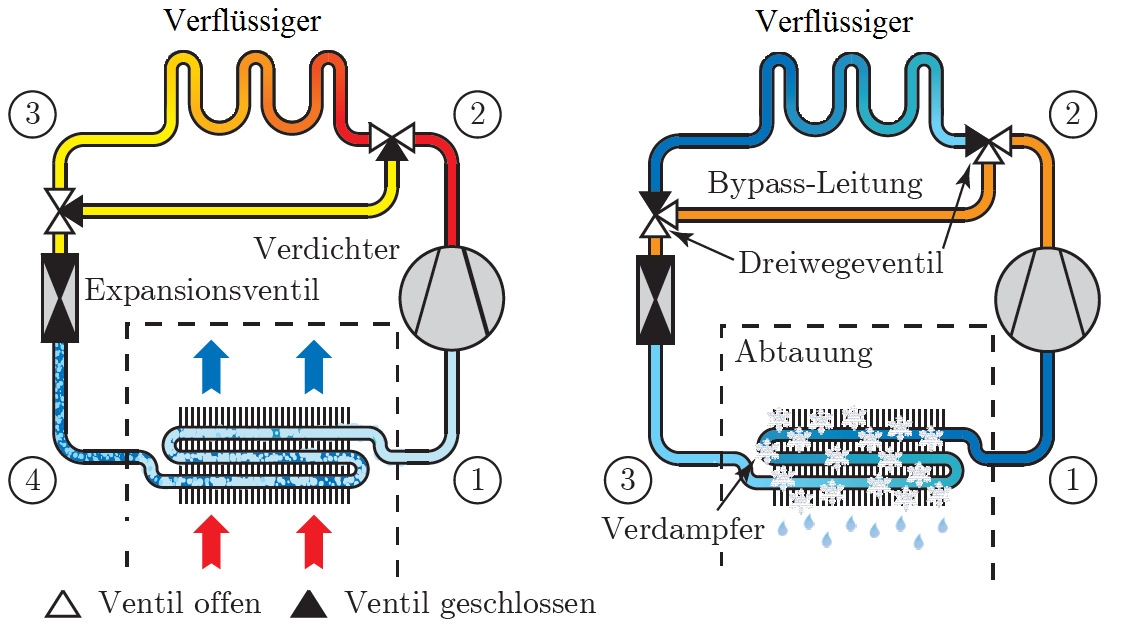
\includegraphics[width=0.640\textwidth]{Pictures/HeissgasKosowski.png}}
\subfigure[Zustandspunkte im log p,h Diagramm]{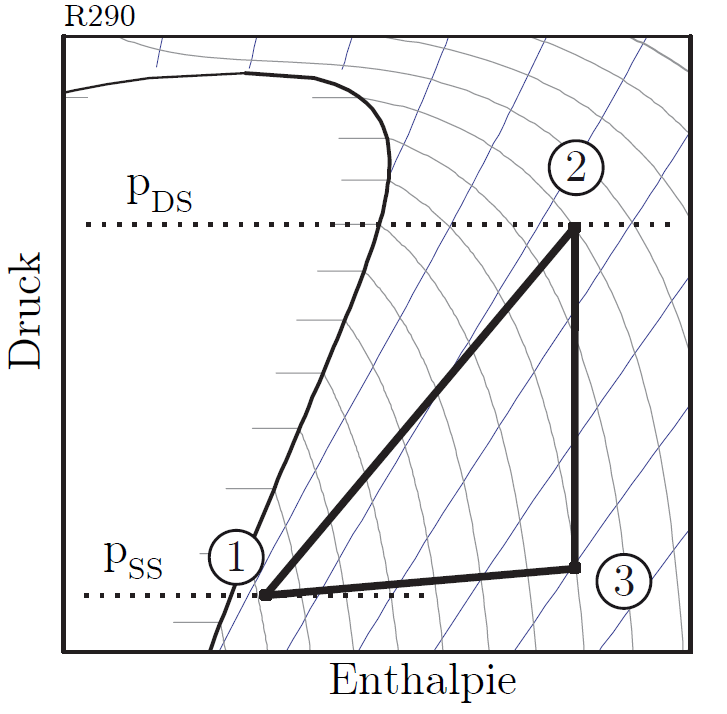
\includegraphics[width=0.35\textwidth]{Pictures/HeissgasEnthalpieDiagrammKosowski.png}}
\caption{Heißgas-Abtauung \citep{Kosowski2009}}
\label{fig:Heissgas-Abtauung}
\end{figure}



\subsection*{Prozessumkehrung}

Bei der Abtauung durch Prozessumkehrung wird die Funktion der Wärmeübertrager vertauscht. Während des Abtauprozesses fungiert der Verdampfer als Verflüssiger und der Verflüssiger hat die Aufgabe des Verdampfers inne. Die Prozessumkehrung wird in der Regel durch ein Vierwegeventil realisiert. Das Vierwegeventil wird bei der Abtauung geschaltet und leitet das Kältemittel nach dem Kompressor erst in den vereisten Verdampfer. Das überhitzte Kältemittel durchströmt den Verdampfer auf hohem Druckniveau und gibt Wärme an die Rohre und Lamellen des Luftkühlers sowie an das Eis ab.

Die Versuchsanlage, die in dieser Arbeit optimiert worden ist, ist mit dieser Technologie ausgestattet. Der Umkehrprozess wird näher im Kapitel \ref{cha: Versuchsaufbau} erläutert. 


\begin{figure}[htb]
\centering		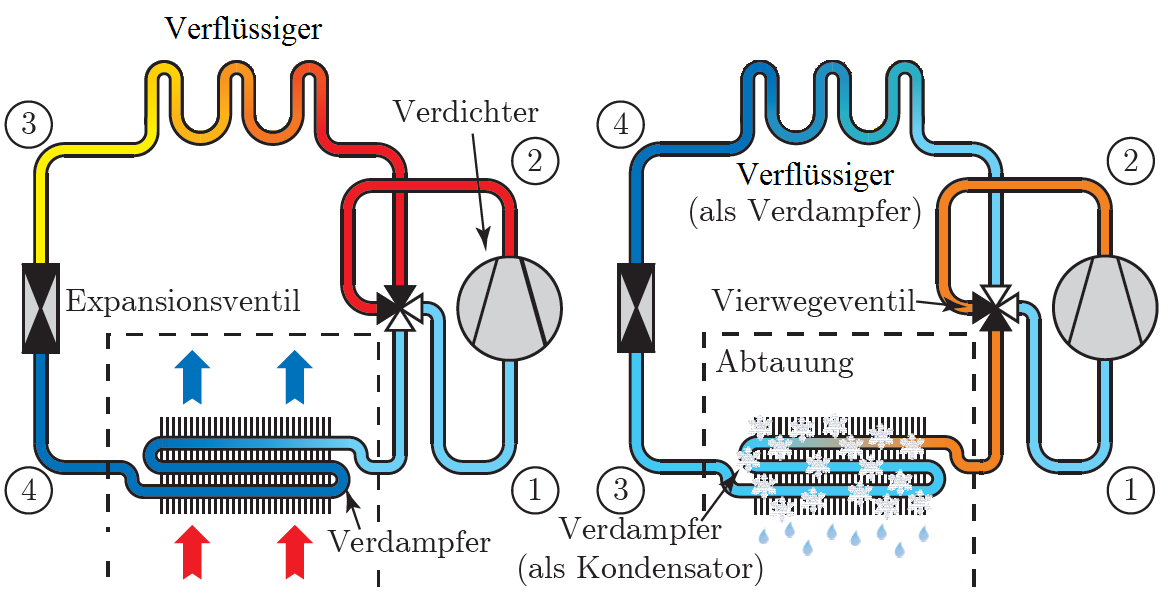
\includegraphics[width=0.7\textwidth]{Pictures/Prozessumkehrung_Kosowski.png}
\caption{Links: Kühlbetrieb. Rechts: Heißgas-Abtauung \citep{Kosowski2009}}
\label{fig:Prozessumkehrung}
\end{figure}

\subsection*{Elektrische Abtauung}

Eine weitere Möglichkeit der Abtauung ist die elektrische Abtauung. Bei dieser Methode sind Widerstandsheizungselemente in den Wärmeübertrager des Verdampfers installiert. Die Widerstandsheizung wandelt elektrische Energie in thermische Energie um und überträgt diese weiter an den Wärmeübertrager und das Eis. 

%Das Prinzip der Widerstandsheizung beruht auf einen niedrig ohmigen Widerstand, der von Strom durchflossen wird und sich dabei erhitzt. Die Widerstandsheizung, auch Heizpatronen genannt, können in Reihe oder auch parallel geschaltet werden.  Die bei der Erhitzung abfallende elektrische Spannung über einen Heizwiderstand errechnet sich nach dem Ohmischen-Gesetz zu :

%\begin{equation}
%U = R I
%\label{eq: Ohmisches Gesetz}
%\end{equation}

%Hierbei ist $R$ der spezifische Widerstand des eingesetzten Materials, meistens Metalle,  und $I$ die angelegte Stromstärke. Ein Heizwiderstand hat einen Wirkungsgrad von 100 $\%$ und wandelt somit die komplette elektrische Leistung in thermische um:

%\begin{equation}
%\dot{Q}_{th}= P_{el }= U I = \frac{U^2}{R} =  R I^2 
%\label{eq:Leistung Heizwiderstand}
%\end{equation}

%Die thermische Leistung ist folglich proportional zu der angelegten Spannung $U$. Die Widerstände sind über die Spannung $U$ regelbar. Der Wärmeübergang von den Heizpatronen auf den Wärmeübertrager ist entscheidend für ein effizientes Abtausystem. Je formschlüssiger die Heizpatronen in den Verdampfer installiert sind, desto besser der Wärmeübergang und effizienter die Abtauuung.  
Die Versuchsanlage dieser Arbeit ist auch mit dieser Abtautechnologie ausgestattet. 

\subsection*{Umluft-Abtauung}

Die Umluft-Abtauung ist eine weitere in der Praxis häufig verwendete Abtaumethode. Hierbei wird der Verdampfer durch die vorbeiströmende Umluft abgetaut. Um dies zu ermöglichen, muss zum einen der Ventilator in der Abtauphase laufen und zum anderen die Umgebungstemperatur größer als 0 °C sein. Ein Vorteil dieses Verfahrens ist, dass die Wärmeübertragung luftseitig geschieht und dadurch die zuzuführende Wärme nicht zusätzlich das Material des Verdampfers erhitzen muss. 

Diese Abtaumethode wird in der Arbeit nicht näher untersucht. Deswegen wird an dieser Stelle auf die  Literaturquellen \citep{Breidenbach2014} und \citep{Ehrbar2002} verwiesen. 

\subsection*{Gegenüberstellung der Abtaumethoden}
\label{subsec:Gegenüberstellung }

Die Tabelle \ref{tab:Vor- und Nachteile} gibt einen Überblick über die Vor- und Nachteile der jeweiligen Abtaumethode. 

\begin{table}%[htb]
\centering
\caption{Vor- und Nachteile der verschiedenen Abtaumethoden   	\citep{Breidenbach2014}, \citep{Refrigeration2000}, \citep{Yin2012}, \citep{Huang20091697}
} \vspace{6pt}

\label{fig:PCM_Slurry1}
%\begin{tabular}{p{3.9cm}p{8cm}p{8cm}lll} 
\begin{tabular}{p{3.8cm}p{5.6cm}p{5.6cm}lll}
\hline
\textbf{Abtaumethode} &\textbf{Vorteile} & \textbf{Nachteile}\\
\hline
\hline

\textbf{Heißgas-Abtauung} 
&
$\bullet$ Guter Wärmeübergang zwischen Heißgas,Rohre und Eis
\newline								  			
$\bullet$ Unkomplizierte Wartung
\newline			  
$\bullet$ Kurze Abtaudauer		
\newline			
$\bullet$ Schnelles Wiederanfahren möglich	

&$\bullet$ Höherer Planungs- und Installationsaufwand  
\newline
$\bullet$ Zusätzliche Kühlung des Kompressors in Abtauphase ist erforderlich 
\newline 
$\bullet$ Höhere Druckverluste durch zusätzliche Komponenten 
\newline
$\bullet$ kritische Kältemittel-Menge bestimmt durch Abtauleistung \\  
   
\hline
\textbf{Prozessumkehrung}
&$\bullet$ Guter Wärmeübergang zwischen Heißgas,Rohre und Eis  													
\newline								
$\bullet$ Unkomplizierte Wartung
\newline	
$\bullet$ Kurze Abtaudauer		
\newline			 
$\bullet$ geeignet für Verbund-Systeme		
&$\bullet$ Abtropfwanne ist nicht beheizt   
\newline
$\bullet$ Höherer Planungs- und Installationsaufwand
\newline
$\bullet$ Nicht nachrüstbar
\newline
$\bullet$ Höhere Druckverluste durch zusätzliche Komponenten								
\newline
$\bullet$ Kritische Kältemittel-Menge bestimmt durch Abtauleistung\\


\hline
\textbf{Elektrische Abtauung }
&$\bullet$ Günstig 
\newline 
$\bullet$ \textit{Stand-Alone}-System ist nachrüstbar		
\newline
$\bullet$ Hohe Regelgenauigkeit	
\newline
$\bullet$ Abtropfwanne ist beheizbar 					
&
$\bullet$ Schlechter Wärmeübergang 
\newline					
$\bullet$ Verursacht Kältemittelbewegung in den Sammler
\newline 
$\bullet$ Brandgefahr im Falle von Kabelbruch  
\newline
$\bullet$ Zeitliche Verzögerung beim Abtauprozess 
\newline
$\bullet$ Hohe thermische Belastung der Komponenten    
\\

 
\hline
\textbf{Umluft-Abtauung }
&
$\bullet$	Keine zusätzlichen Komponenten nötig			 
\newline
$\bullet$	Günstig										
\newline
$\bullet$	Keine zusätzlicher Wärmeeintrag ins System	  
\newline
$\bullet$	Keine Abtauung der Abtauwanne möglich	
&
$\bullet$ Bei überdimensionierten Kompressoren sehr hohe Abtaudauer möglich
\newline
$\bullet$ Funktioniert nur mit Umgebungstemperaturen über $ 2\,^{\circ}\mathrm{C} $
\\
\hline

\end{tabular}
\label{tab:Vor- und Nachteile}
\end{table}
%\end{landscape}

